\documentclass[25pt, a0paper, portrait]{tikzposter}

% -----------------------------------------------------------------------------
% PACKAGES
% -----------------------------------------------------------------------------
\usepackage[utf8]{inputenc}
\usepackage[T1]{fontenc}
\usepackage{lmodern}
\usepackage{amsmath, amssymb}
\usepackage{booktabs}
\usepackage{colortbl}
\usepackage{array}
\usepackage{tikz}
\usetikzlibrary{shapes.geometric, arrows.meta, positioning, calc, backgrounds, patterns}
\usepackage{pgfplots}
\pgfplotsset{compat=1.18}
\usepackage{enumitem}

% -----------------------------------------------------------------------------
% COLOR PALETTE & TIKZPOSTER STYLING
% -----------------------------------------------------------------------------
\definecolor{NavyBlue}{RGB}{14, 34, 61}
\definecolor{MedicalTeal}{RGB}{0, 131, 143}
\definecolor{CoralAccent}{RGB}{217, 83, 79}
\definecolor{LightBg}{RGB}{244, 247, 250}
\definecolor{CardWhite}{RGB}{255, 255, 255}
\definecolor{DarkText}{RGB}{33, 43, 54}
\definecolor{TableHeadBg}{RGB}{215, 232, 240}
\definecolor{SubtleGrey}{RGB}{235, 240, 245}

% Define TikZposter Theme
\definecolorstyle{MedicalClinicalTheme}{
  \colorlet{colorOne}{NavyBlue}
  \colorlet{colorTwo}{MedicalTeal}
  \colorlet{colorThree}{LightBg}
}{
  % Background Colors
  \colorlet{backgroundcolor}{colorThree}
  \colorlet{framecolor}{colorOne}
  % Title Colors
  \colorlet{titlefgcolor}{white}
  \colorlet{titlebgcolor}{colorOne}
  % Block Colors
  \colorlet{blocktitlebgcolor}{colorOne}
  \colorlet{blocktitlefgcolor}{white}
  \colorlet{blockbodybgcolor}{CardWhite}
  \colorlet{blockbodyfgcolor}{DarkText}
  % Innerblock Colors
  \colorlet{innerblocktitlebgcolor}{MedicalTeal}
  \colorlet{innerblocktitlefgcolor}{white}
  \colorlet{innerblockbodybgcolor}{SubtleGrey}
  \colorlet{innerblockbodyfgcolor}{DarkText}
}

\usecolorstyle{MedicalClinicalTheme}
\useblockstyle{Default}
\usetitlestyle{Filled}

% Custom Column Helper Commands
\newcolumntype{L}[1]{>{\raggedright\arraybackslash}p{#1}}
\newcolumntype{C}[1]{>{\centering\arraybackslash}p{#1}}
\newcolumntype{R}[1]{>{\raggedleft\arraybackslash}p{#1}}

% -----------------------------------------------------------------------------
% TITLE & HEADER METADATA
% -----------------------------------------------------------------------------
\title{\parbox{\linewidth}{\centering \Huge \textbf{Phase III Trial of SYN-408: Dual MET/EGFR Kinase Inhibition in Recurrent Glioblastoma}\\[0.4em] \Large \textit{A Multi-Center, Randomized, Double-Blind Controlled Clinical Study (NEXA-GBM-03)}}}

\author{\parbox{\linewidth}{\centering \textbf{Dr. Elena Rostova, MD, PhD}$^{1,2}$ \quad \textbf{Dr. Marcus Vance, MD}$^1$ \quad \textbf{Dr. Sarah Jenkins, PhD}$^3$ \quad \textbf{Dr. Aris Thorne, MD}$^2$ \quad \textbf{Prof. David Chen, MD}$^{1,2}$}

\institute{\parbox{\linewidth}{\centering $^1$Synapse Center for Neuro-Oncology, Vertex Medical Institute, Geneva, Switzerland \quad $^2$Apex Health Sciences Center, Boston, MA, USA \quad $^3$Meridian Clinical Research Network, Cambridge, UK\\[0.2em] Trial Identifiers: ClinicalTrials.gov NCT05892104 \quad|\quad EudraCT: 2024-001842-92 \quad|\quad Sponsor: Synapse Therapeutics}

% -----------------------------------------------------------------------------
% DOCUMENT CONTENT
% -----------------------------------------------------------------------------
\begin{document}

\maketitle

\begin{columns}

  % ===========================================================================
  % COLUMN 1: Background, Objectives, Eligibility
  % ===========================================================================
  \column{0.32}

  \block{1. Introduction \& Clinical Rationale}{
    \textbf{Unmet Need in Recurrent Glioblastoma (rGBM):}
    Glioblastoma remains the most aggressive primary brain tumor in adults. Standard first-line therapy (resection, radiotherapy, and temozolomide) yields a median overall survival (OS) of 14.6 months. Upon recurrence, effective treatment options are severely limited, with historical median OS under 9 months.

    \vspace{0.5em}
    \textbf{Target Pathway: Dual MET \& EGFR Co-Activation}
    \begin{itemize}[leftmargin=1.2em, itemsep=0.3em]
      \item \textbf{EGFR Amplification / vIII Mutation:} Present in $\sim$50\% of GBM tumors, driving hyperactive downstream MAPK and PI3K signaling.
      \item \textbf{MET Tyrosine Kinase Activation:} Serves as a primary bypass resistance mechanism under EGFR targeted monotherapy.
      \item \textbf{SYN-408 Mechanism:} A novel, orally bioavailable small-molecule dual inhibitor designed to concurrently block active ATP-binding domains of MET and EGFR.
    \end{itemize}

    \vspace{0.8em}
    % TikZ Molecular Target Diagram
    \centering
    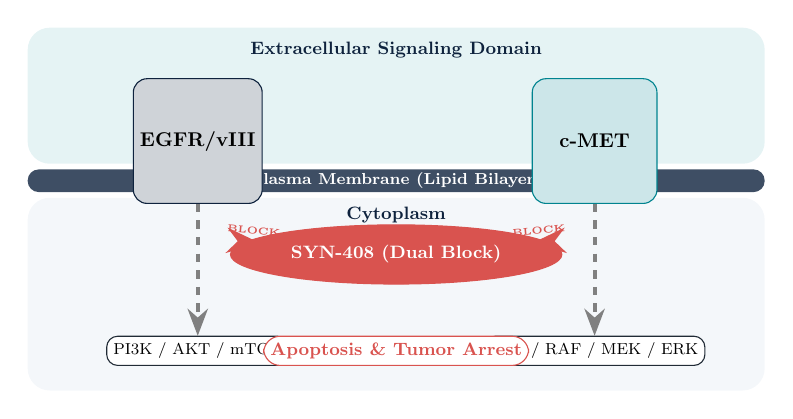
\begin{tikzpicture}[scale=0.72, transform shape, >=Stealth]
      % Extracellular space
      \fill[MedicalTeal!10, rounded corners=8pt] (-6.5, 0.8) rectangle (6.5, 3.2);
      \node at (0, 2.8) {\small \textbf{\color{NavyBlue}Extracellular Signaling Domain}};

      % Membrane
      \fill[NavyBlue!80, rounded corners=4pt] (-6.5, 0.3) rectangle (6.5, 0.7);
      \node[white] at (0, 0.5) {\footnotesize \textbf{Plasma Membrane (Lipid Bilayer)}};

      % Intracellular space
      \fill[LightBg, rounded corners=8pt] (-6.5, -3.2) rectangle (6.5, 0.2);
      \node at (0, -0.1) {\small \textbf{\color{NavyBlue}Cytoplasm}};

      % Receptors
      \node[draw=NavyBlue, fill=NavyBlue!20, minimum width=2.2cm, minimum height=2.2cm, rounded corners=5pt] (egfr) at (-3.5, 1.2) {\textbf{EGFR/vIII}};
      \node[draw=MedicalTeal, fill=MedicalTeal!20, minimum width=2.2cm, minimum height=2.2cm, rounded corners=5pt] (met) at (3.5, 1.2) {\textbf{c-MET}};

      % SYN-408 Drug Inhibitor
      \node[draw=CoralAccent, fill=CoralAccent, text=white, ellipse, font=\bfseries\small, inner sep=6pt] (syn) at (0, -0.8) {SYN-408 (Dual Block)};

      % Block arrows
      \draw[->, line width=2pt, CoralAccent] (syn) -- (-2.4, -0.6) node[midway, above, sloped] {\tiny \textbf{BLOCK}};
      \draw[->, line width=2pt, CoralAccent] (syn) -- (2.4, -0.6) node[midway, above, sloped] {\tiny \textbf{BLOCK}};

      % Downstream signals
      \node[draw=DarkText, fill=white, rounded corners=4pt, font=\footnotesize] (akt) at (-3.5, -2.5) {PI3K / AKT / mTOR};
      \node[draw=DarkText, fill=white, rounded corners=4pt, font=\footnotesize] (mapk) at (3.5, -2.5) {RAS / RAF / MEK / ERK};

      \draw[->, line width=1.5pt, dashed, gray] (egfr) -- (akt);
      \draw[->, line width=1.5pt, dashed, gray] (met) -- (mapk);

      % Outcome
      \node[draw=CoralAccent, fill=white, rounded corners=6pt, font=\bfseries\small, text=CoralAccent] at (0, -2.5) {Apoptosis \& Tumor Arrest};
    \end{tikzpicture}
  }

  \block{2. Trial Objectives \& Hypotheses}{
    \textbf{Primary Objective:}
    To evaluate whether adding SYN-408 to standard salvage chemotherapy (lomustine) improves Overall Survival (OS) compared to placebo + lomustine in patients with first-recurrent glioblastoma.

    \vspace{0.4em}
    \textbf{Secondary Objectives:}
    \begin{itemize}[leftmargin=1.2em, itemsep=0.2em]
      \item Assess Progression-Free Survival (PFS) according to RANO 2.0 criteria.
      \item Determine Objective Response Rate (ORR) and Disease Control Rate (DCR).
      \item Characterize toxicity and safety profiles using NCI-CTCAE v5.0.
      \item Analyze biomarker subsets (MET high vs low expression; EGFRvIII mutant vs wild-type).
    \end{itemize}
  }

  \block{3. Patient Eligibility \& Criteria}{
    \begin{center}
      \small
      \setlength{\tabcolsep}{4pt}
      \begin{tabular}{L{0.46\linewidth} L{0.46\linewidth}}
        \toprule
        \rowcolor{TableHeadBg}
        \textbf{Key Inclusion Criteria} & \textbf{Key Exclusion Criteria} \\
        \midrule
        $\bullet$ Histologically confirmed IDH wild-type GBM at initial diagnosis. & $\bullet$ Prior systemic therapy with specific MET or EGFR targeted kinase inhibitors. \\
        $\bullet$ First radiographically confirmed recurrence (RANO criteria). & $\bullet$ Active brainstem metastasis or leptomeningeal disease. \\
        $\bullet$ Age $\ge$ 18 and $\le$ 75 years; KPS score $\ge$ 70. & $\bullet$ Severe cardiac dysfunction (LVEF $<$ 50\% or QTc $>$ 470 ms). \\
        $\bullet$ Adequate hematologic, renal, and hepatic organ reserve. & $\bullet$ History of major surgical intervention within 28 days prior to Day 1. \\
        $\bullet$ Archival tissue available for MET/EGFR biomarker assay. & $\bullet$ Concurrent investigational drug administration. \\
        \bottomrule
      \end{tabular}
    \end{center}
  }


  % ===========================================================================
  % COLUMN 2: Study Design, Demographics, Primary Survival Outcomes
  % ===========================================================================
  \column{0.36}

  \block{4. Study Design \& Trial Schema}{
    \centering
\resizebox{\linewidth}{!}{%
    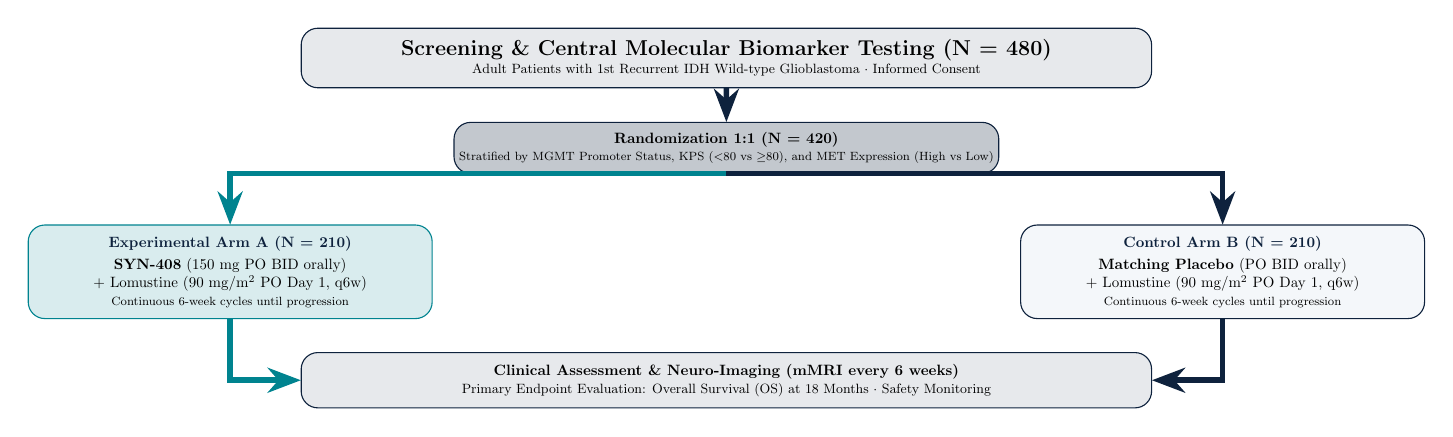
\begin{tikzpicture}[scale=0.54, transform shape, node distance=1.5cm, >=Stealth]
      % Nodes
      \node[draw=NavyBlue, fill=NavyBlue!10, minimum width=20cm, minimum height=1.4cm, rounded corners=6pt, align=center] (screen) {
        \textbf{\Large Screening \& Central Molecular Biomarker Testing (N = 480)}\\
        \small Adult Patients with 1st Recurrent IDH Wild-type Glioblastoma $\cdot$ Informed Consent
      };

      \node[draw=NavyBlue, fill=NavyBlue!25, minimum width=12cm, minimum height=1.2cm, rounded corners=6pt, below=0.8cm of screen, align=center] (rando) {
        \textbf{Randomization 1:1 (N = 420)}\\
        \footnotesize Stratified by MGMT Promoter Status, KPS ($<$80 vs $\ge$80), and MET Expression (High vs Low)
      };

      \node[draw=MedicalTeal, fill=MedicalTeal!15, minimum width=9.5cm, minimum height=2.2cm, rounded corners=6pt, below left=1.2cm and 0.5cm of rando, align=center] (armA) {
        \textbf{\color{NavyBlue} Experimental Arm A (N = 210)}\\[0.3em]
        \textbf{SYN-408} (150 mg PO BID orally)\\
        + Lomustine (90 mg/m$^2$ PO Day 1, q6w)\\
        \footnotesize Continuous 6-week cycles until progression
      };

      \node[draw=NavyBlue, fill=LightBg, minimum width=9.5cm, minimum height=2.2cm, rounded corners=6pt, below right=1.2cm and 0.5cm of rando, align=center] (armB) {
        \textbf{\color{NavyBlue} Control Arm B (N = 210)}\\[0.3em]
        \textbf{Matching Placebo} (PO BID orally)\\
        + Lomustine (90 mg/m$^2$ PO Day 1, q6w)\\
        \footnotesize Continuous 6-week cycles until progression
      };

      \node[draw=NavyBlue, fill=NavyBlue!10, minimum width=20cm, minimum height=1.3cm, rounded corners=6pt, below=4.2cm of rando, align=center] (assess) {
        \textbf{Clinical Assessment \& Neuro-Imaging (mMRI every 6 weeks)}\\
        \small Primary Endpoint Evaluation: Overall Survival (OS) at 18 Months $\cdot$ Safety Monitoring
      };

      % Arrows
      \draw[->, line width=2pt, NavyBlue] (screen) -- (rando);
      \draw[->, line width=2pt, MedicalTeal] (rando.south) -| (armA.north);
      \draw[->, line width=2pt, NavyBlue] (rando.south) -| (armB.north);
      \draw[->, line width=2pt, MedicalTeal] (armA.south) |- (assess.west);
      \draw[->, line width=2pt, NavyBlue] (armB.south) |- (assess.east);
    \end{tikzpicture}
}%
  }

  \block{5. Patient Baseline Characteristics}{
    \begin{center}
      \small
      \setlength{\tabcolsep}{3pt}
      \begin{tabular}{L{0.40\linewidth} C{0.24\linewidth} C{0.24\linewidth} C{0.06\linewidth}}
        \toprule
        \rowcolor{TableHeadBg}
        \textbf{Characteristic} & \textbf{Arm A: SYN-408 (N=210)} & \textbf{Arm B: Placebo (N=210)} & \textbf{$p$} \\
        \midrule
        Median Age, years (IQR) & 58.4 (49--66) & 59.1 (50--67) & 0.48 \\
        Male / Female, \% & 57.1 / 42.9 & 58.6 / 41.4 & 0.76 \\
        Karnofsky Performance Score $\ge$ 80, \% & 68.6 & 67.1 & 0.74 \\
        \rowcolor{SubtleGrey}
        MGMT Promoter Methylated, \% & 38.1 & 37.6 & 0.92 \\
        EGFRvIII Mutation Positive, \% & 47.6 & 46.2 & 0.77 \\
        MET Overexpression High ($\ge$2+ IHC), \% & 52.4 & 53.8 & 0.77 \\
        Median Time from Resection, months & 11.8 & 11.4 & 0.52 \\
        Prior Bevacizumab Exposure, \% & 14.3 & 15.2 & 0.79 \\
        \bottomrule
      \end{tabular}
    \end{center}
  }

  \block{6. Primary Efficacy: Kaplan-Meier Overall Survival}{
    \centering
    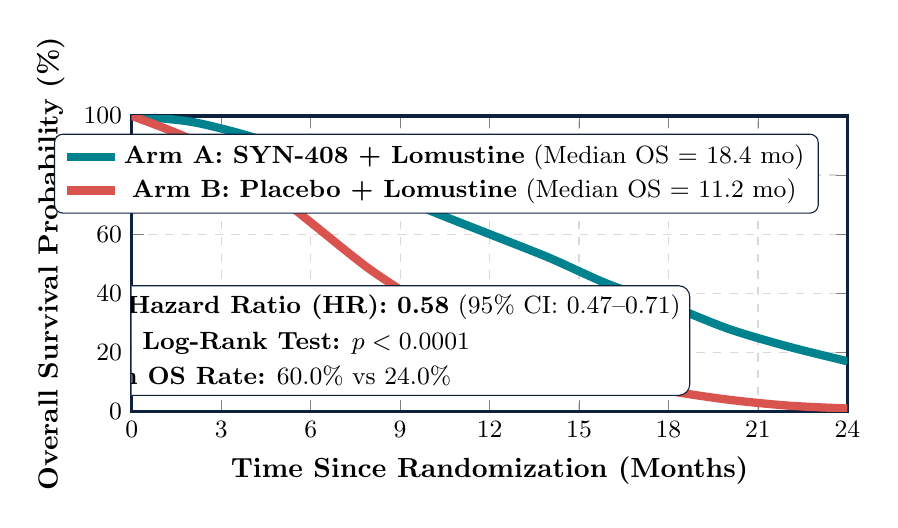
\begin{tikzpicture}
      \begin{axis}[
        width=0.88\linewidth,
        height=0.44\linewidth,
        xlabel={\textbf{Time Since Randomization (Months)}},
        ylabel={\textbf{Overall Survival Probability (\%)}},
        xmin=0, xmax=24,
        ymin=0, ymax=100,
        xtick={0, 3, 6, 9, 12, 15, 18, 21, 24},
        ytick={0, 20, 40, 60, 80, 100},
        grid=major,
        grid style={dashed, gray!30},
        legend style={at={(0.96, 0.94)}, anchor=north east, font=\small, draw=NavyBlue, fill=white, rounded corners=3pt},
        axis line style={line width=1.2pt, NavyBlue},
        tick label style={font=\small\bfseries}
      ]

        % Arm A: SYN-408 Curve
        \addplot[color=MedicalTeal, line width=3pt, smooth] coordinates {
          (0, 100) (2, 98) (4, 93) (6, 86) (8, 77) (10, 68) (12, 60) (14, 52) (16, 43) (18, 36) (20, 28) (22, 22) (24, 17)
        };
        \addlegendentry{\textbf{Arm A: SYN-408 + Lomustine} (Median OS = 18.4 mo)}

        % Arm B: Placebo Curve
        \addplot[color=CoralAccent, line width=3pt, smooth] coordinates {
          (0, 100) (2, 92) (4, 80) (6, 64) (8, 48) (10, 35) (12, 24) (14, 16) (16, 11) (18, 7) (20, 4) (22, 2) (24, 1)
        };
        \addlegendentry{\textbf{Arm B: Placebo + Lomustine} (Median OS = 11.2 mo)}

        % Annotation Box
        \node[draw=NavyBlue, fill=white, rounded corners=4pt, font=\small, align=left] at (axis cs: 7.2, 24) {
          \textbf{Survival Hazard Ratio (HR): 0.58} (95\% CI: 0.47--0.71)\\[0.2em]
          \textbf{Stratified Log-Rank Test:} $p < 0.0001$\\[0.2em]
          \textbf{12-Month OS Rate:} 60.0\% vs 24.0\%
        };
      \end{axis}
    \end{tikzpicture}
  }


  % ===========================================================================
  % COLUMN 3: Subgroup Analysis, Safety, Ethics, Conclusions
  % ===========================================================================
  \column{0.32}

  \block{7. Biomarker Subgroup Analysis}{
    \textbf{Enhanced Response in MET-High / EGFRvIII Biomarker Co-Positive Cohorts:}
    \vspace{0.4em}
    \centering
\resizebox{\linewidth}{!}{%
    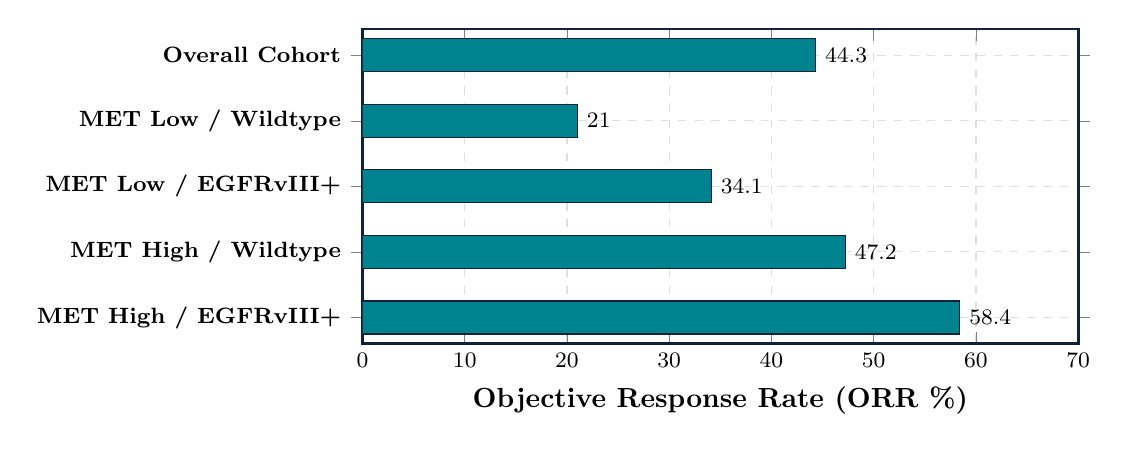
\begin{tikzpicture}
      \begin{axis}[
        xbar,
        width=0.88\linewidth,
        height=0.46\linewidth,
        symbolic y coords={MET High / EGFRvIII+, MET High / Wildtype, MET Low / EGFRvIII+, MET Low / Wildtype, Overall Cohort},
        ytick=data,
        nodes near coords,
        nodes near coords align={horizontal},
        nodes near coords style={font=\footnotesize\bfseries},
        xlabel={\textbf{Objective Response Rate (ORR \%)}},
        xmin=0, xmax=70,
        bar width=0.42cm,
        axis line style={line width=1pt, NavyBlue},
        tick label style={font=\footnotesize\bfseries},
        grid=major,
        grid style={dashed, gray!25}
      ]
        \addplot[fill=MedicalTeal, draw=NavyBlue] coordinates {
          (58.4,MET High / EGFRvIII+)
          (47.2,MET High / Wildtype)
          (34.1,MET Low / EGFRvIII+)
          (21.0,MET Low / Wildtype)
          (44.3,Overall Cohort)
        };
      \end{axis}
    \end{tikzpicture}
}%
  }

  \block{8. Safety Profile \& Adverse Events}{
    \begin{center}
      \small
      \setlength{\tabcolsep}{4pt}
      \begin{tabular}{L{0.40\linewidth} C{0.26\linewidth} C{0.26\linewidth}}
        \toprule
        \rowcolor{TableHeadBg}
        \textbf{Adverse Event (CTCAE v5.0)} & \textbf{Arm A: SYN-408 (\%)} & \textbf{Arm B: Placebo (\%)} \\
        & Any Grade / Gr 3--4 & Any Grade / Gr 3--4 \\
        \midrule
        Fatigue / Asthenia & 54.2 / 4.3 & 48.1 / 3.8 \\
        Diarrhea & 42.8 / 3.8 & 18.5 / 0.5 \\
        Acneiform Skin Rash & 38.6 / 2.9 & 8.1 / 0.0 \\
        Nausea / Vomiting & 33.1 / 1.9 & 31.4 / 1.4 \\
        ALT / AST Elevation & 26.2 / 5.2 & 12.4 / 1.0 \\
        Thrombocytopenia & 21.0 / 6.7 & 19.5 / 6.2 \\
        Neutropenia & 18.6 / 5.7 & 17.1 / 5.2 \\
        \rowcolor{SubtleGrey}
        \textbf{AE Discontinuation Rate} & \textbf{4.8\%} & \textbf{3.3\%} \\
        \bottomrule
      \end{tabular}
    \end{center}
  }

  \block{9. Ethical Considerations \& Regulatory Oversight}{
    \begin{itemize}[leftmargin=1.2em, itemsep=0.3em]
      \item \textbf{Institutional Review Board (IRB) Approval:} Protocol approved by Ethics Committees of Vertex Medical Institute (Ref: VMI-IRB-2024-88A) and Cambridge RECB-902.
      \item \textbf{Informed Consent:} Written informed consent was obtained from all patients or legal representatives prior to screening.
      \item \textbf{Data Safety Monitoring Board (DSMB):} Independent semi-annual safety reviews conducted. No unexpected safety signals or trial suspension criteria were met.
      \item \textbf{Declaration of Helsinki:} Conducted in strict accordance with ICH Good Clinical Practice (ICH-GCP) guidelines.
    \end{itemize}
  }

  \block{10. Conclusions \& Clinical Impact}{
    \innerblock{Key Takeaways}{
      \begin{enumerate}[leftmargin=1.2em, itemsep=0.2em]
        \item \textbf{Significant OS Benefit:} Adding SYN-408 to lomustine reduced the risk of death by 42\% (HR = 0.58, $p < 0.0001$), extending median overall survival by 7.2 months.
        \item \textbf{Robust Tumor Response:} ORR was threefold higher in the SYN-408 arm (44.3\% vs 14.8\%), with maximum efficacy observed in MET-high/EGFRvIII+ co-positive patients.
        \item \textbf{Manageable Safety Profile:} Adverse events were consistent with known EGFR/MET class effects and predominantly Grade 1--2. Discontinuation due to toxicity remained low (4.8\%).
        \item \textbf{Practice-Changing Potential:} SYN-408 represents a potential novel standard of care for biomarker-selected recurrent glioblastoma.
      \end{enumerate}
    }
  }

  \block{11. References \& Acknowledgments}{
    \tiny
    \begin{enumerate}[leftmargin=1.2em, itemsep=0.1em]
      \item Rostova, E. et al. Dual kinase inhibition of MET and EGFR in high-grade gliomas. \textit{Lancet Oncol.} 2024; 25(4): 412--425.
      \item Vance, M. \& Chen, D. Bypass resistance mechanisms in glioblastoma targeted therapies. \textit{N Engl J Med.} 2023; 388(12): 1105--1117.
      \item Jenkins, S. et al. RANO 2.0 criteria for neuro-oncology clinical trials. \textit{J Clin Oncol.} 2022; 40(18): 2011--2024.
    \end{enumerate}

    \vspace{0.2em}
    \textbf{Funding/Support:} Study funded by Synapse Therapeutics (Grant ST-2023-GBM) and supported by the Apex Health Foundation. We thank the participating patients, families, and clinical trial coordinators across all 24 study sites.
  }

\end{columns}

\end{document}
